\documentclass[a4paper,12pt,oneside,article]{memoir}


%%%% PACKAGES %%%%

\usepackage[T1]{fontenc}
\usepackage[utf8]{inputenc}
\usepackage{fourier}
\usepackage[danish]{babel}
\usepackage{cleveref}
\usepackage{graphicx}
\graphicspath{{Images/}}

%   ¤¤ Afsnitsformatering ¤¤ %
\setlength{\parindent}{0mm}             % Størrelse af indryk
\setlength{\parskip}{3mm}                   % Afstand mellem afsnit ved brug af double Enter
\linespread{1,2}                                                % Linie afstand
% length of abstract indentations
\setlength{\absleftindent}{0mm}
\setlength{\absrightindent}{0mm} 

\begin{document}

\chapter{Process Analyse}

    \section{Beskrivelse - Hvad gjorde vi i P1} 

        \subsection{Projektplanlægning}

        Der blev lavet undervejs to tidsplaner, med deadlines til f.eks. hvornår vi skulle afslutte problemanalysen. Da ikke alle tidspunkter var realistiske under hele forløbet, blev der lavet en ny iteration.
  
        Der har ikke været en person, der blev udpeget at været projektleder, istedet har vi været meget demokratiske. Tilsidst i projekt forløbet tog nogle gruppemedlem rollen, som projektleder for en dag, hvis rolle var at skulle styr på hvad der var lavet og hvad der stadig manglede at blivet lavet. Beslutninger har været mere enstemmige, men beslutningerne har også først været taget efter længere diskussioner.

            I hvilket omfang har gruppens medlemmer haft samme opfattelse af hvad projektplanlægning indebærer?

            Opfattelsen af projectplanlægning har i gruppen været hovesaglig, Brainstorm, posters og tidsplanlægning. Hvor alle tre ting kan ændre med tiden. Der blev lavet undervejs to tidsplaner, med deadlines til f.eks. hvornår vi skulle afslutte problemanalysen. Da ikke alle tidspunkter var realistiske under hele forløbet, blev der lavet en ny iteration.

            Har I haft nogle projektplaner? I så fald: Hvilke, hvad har I anvendt dem til og hvordan har de fungeret? Hvis ikke: Vil I lave projektplaner i P1? I så fald: Hvilke og hvad vil I bruge dem til?
            
            Inden for den første uge af P1, lavede vi en tids plan for P1, tids blev lavet en tidsplan(ses her under) med poster så der let kunne laves om, eller flyttes rundt på emnerne, hvis vi havde brug for mere tid eller hvis et emne blev færdigt. Hen i slutningen af Projektet blev der lavet  en tidsplan v. 2.0. vores arbejde, er blevet udarbejdet  efter tidsplanen, for at kunne have et overblik over hvad der skulle laves og hvornår det skulle være færdigt.

            \begin{figure}[ht!]
                \centering
                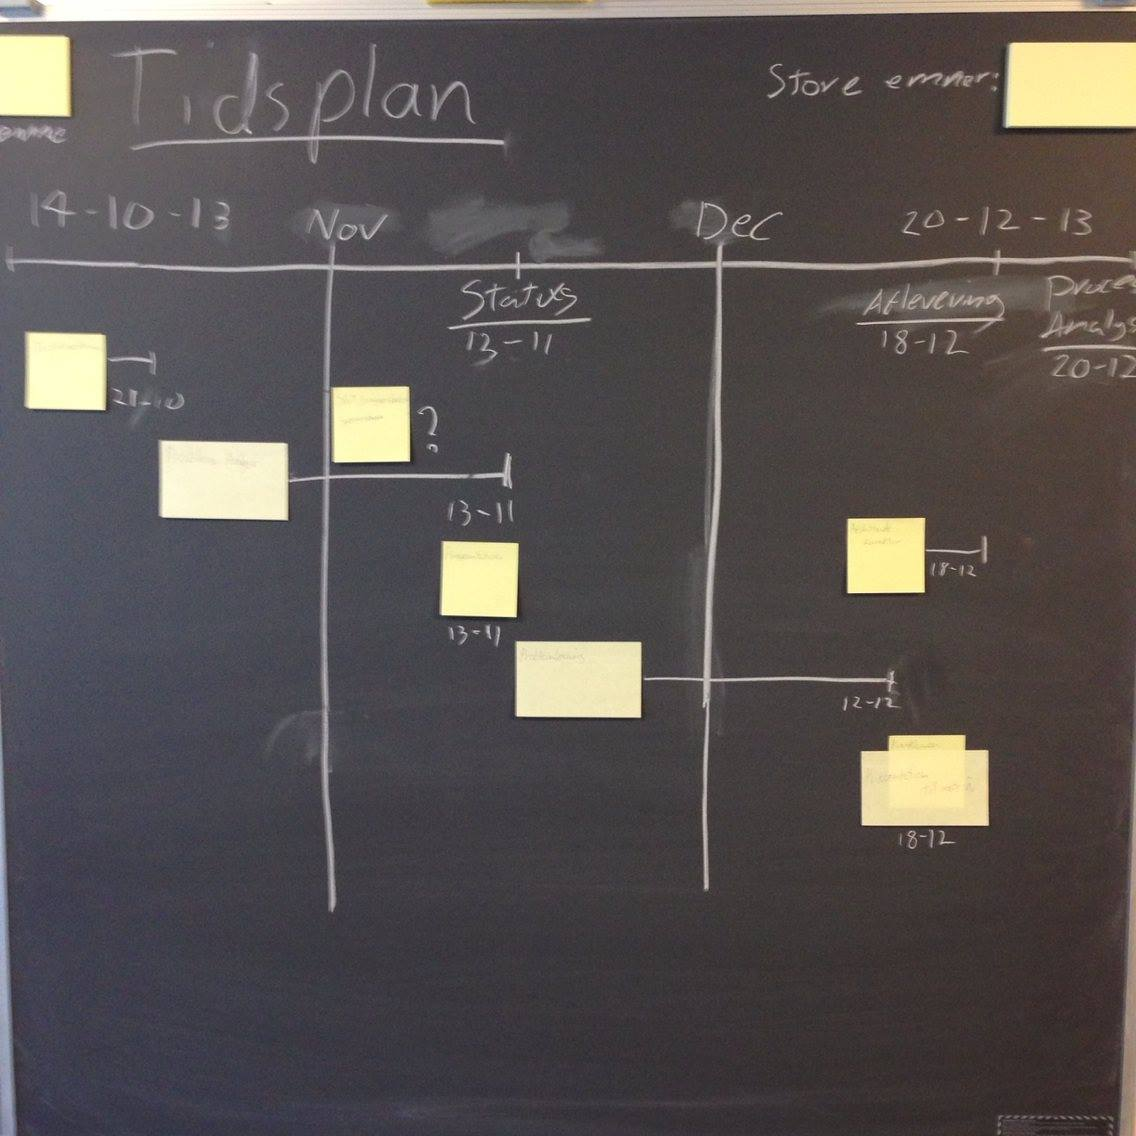
\includegraphics[width=0.5\textwidth]{Images/9.jpg}
                \caption{BAH}
                \label{4}
            \end{figure}

            \begin{figure}[ht!]
                \centering
                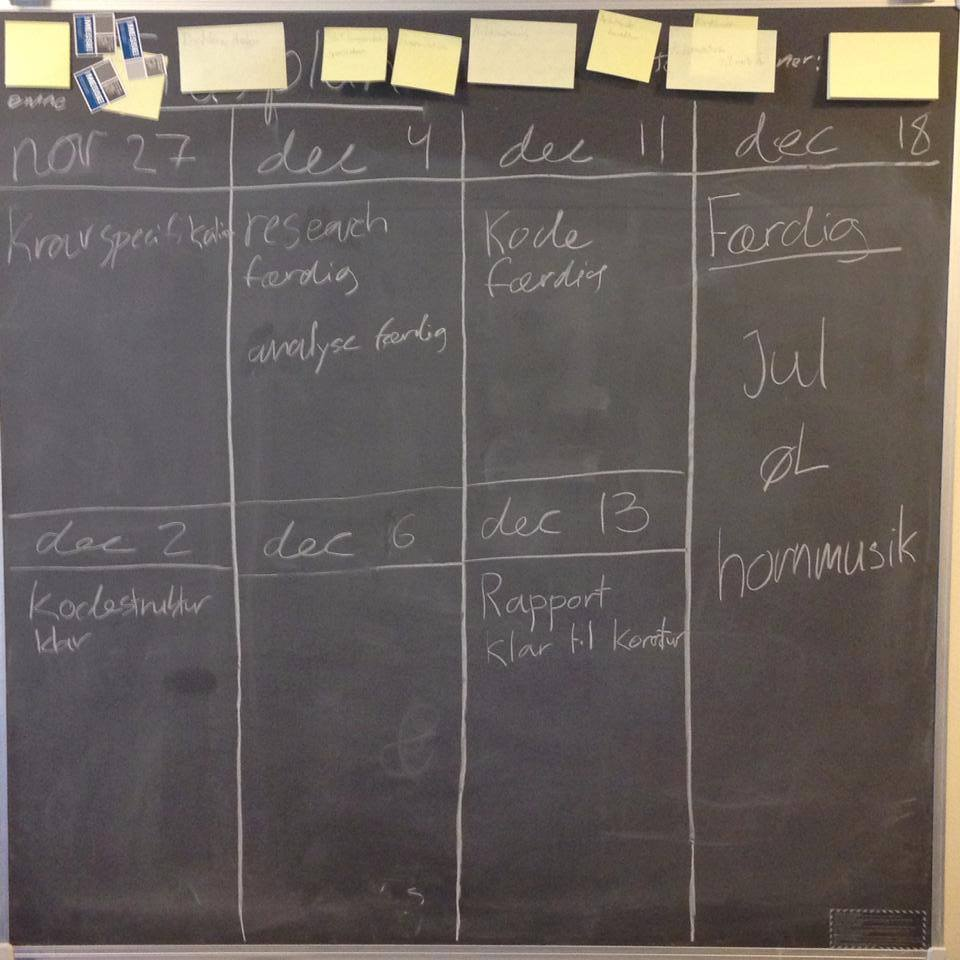
\includegraphics[width=0.5\textwidth]{Images/2.jpg}
                \caption{BAH}
                \label{4}
            \end{figure}

\subsection{Gruppesamarbejde}

En fælles samarbejdsaftale blev lavet \ref{SAftale}, med aftaler om mødetider og regler omkring brugen af software og værktøjer\ref{4}. Aftalen blev lavet i en skriftlig udgave, fordi så kunne man nemmere referer til arket hvis der kom tvivl om hvad der var aftalt. Samt at alle i gruppen kunne skrive under for at vise at de gik med i hvad der var nedskrevet.

\begin{figure}[ht!]
  \centering
  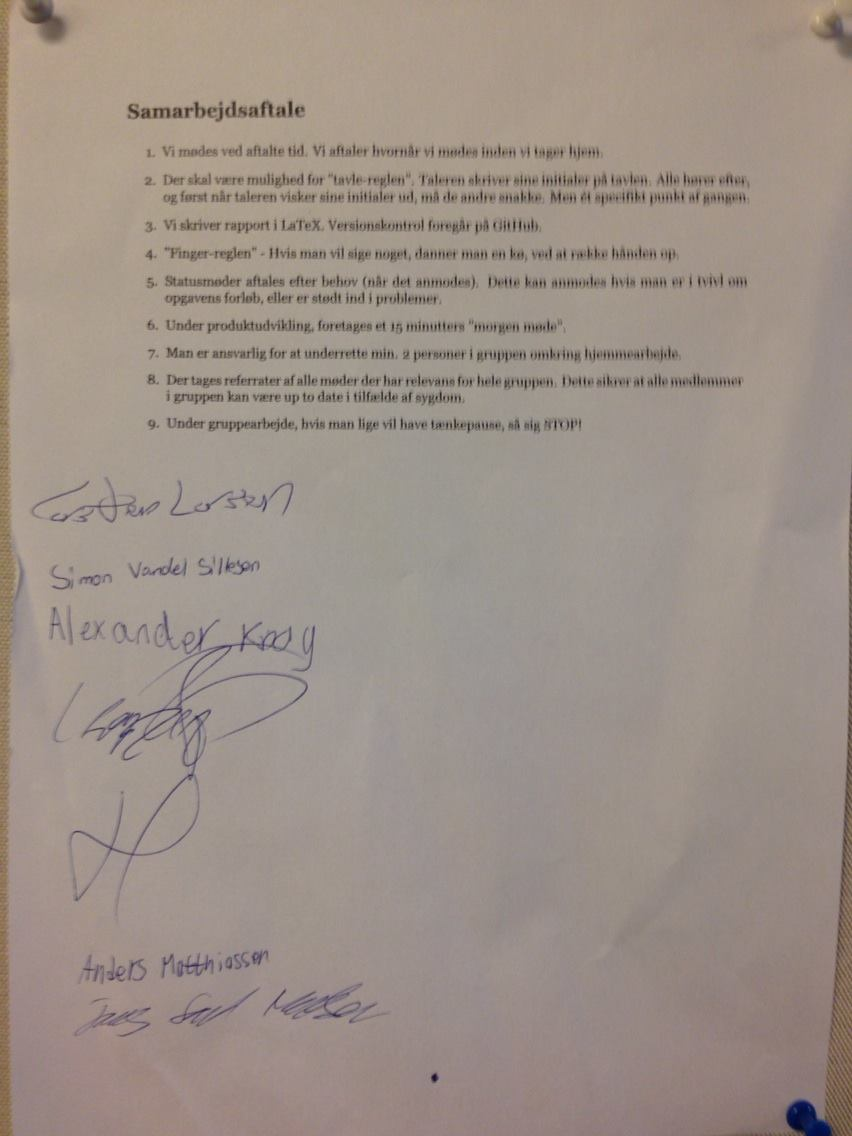
\includegraphics[width=0.5\textwidth]{Images/S_Aftale.jpg}
  \caption{nada}
  \label{SAftale}
\end{figure}

\begin{figure}[ht!]
    \centering
    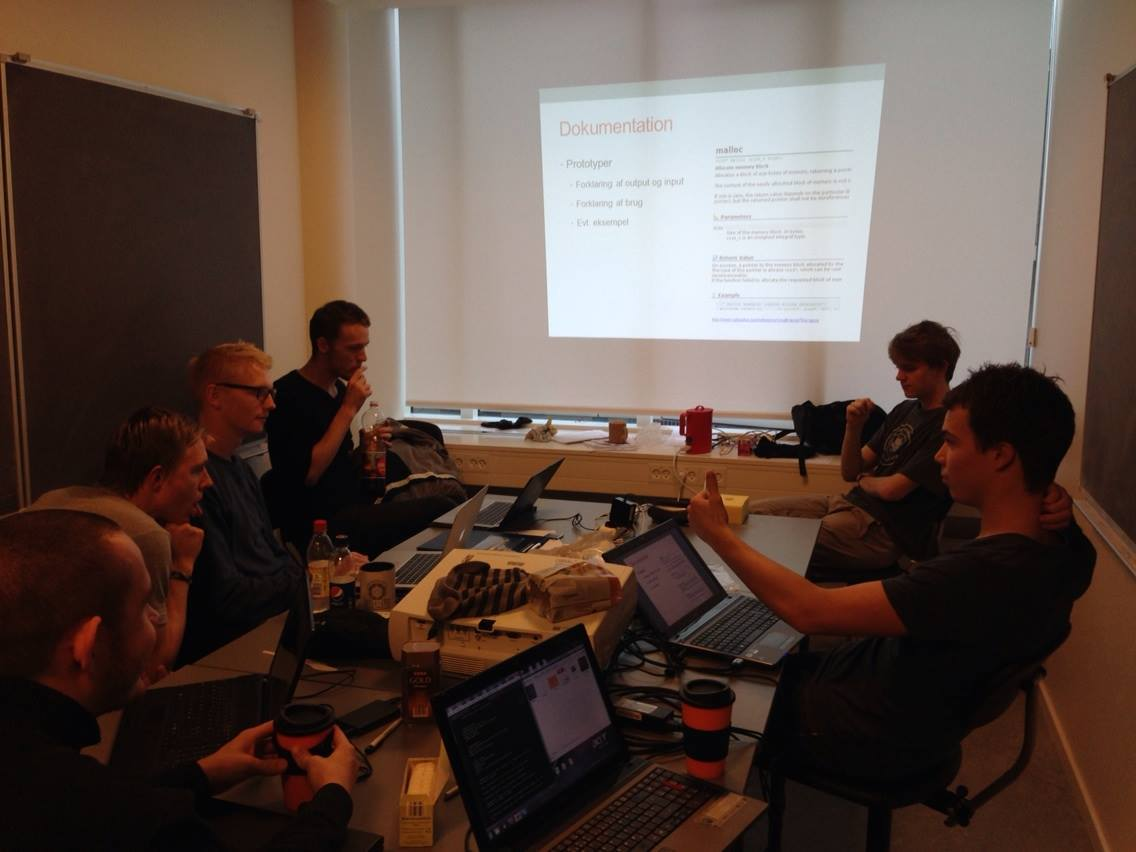
\includegraphics[width=0.5\textwidth]{Images/8.jpg}
    \caption{BAH}
    \label{4}
\end{figure}
Gruppen har været enige om et ambitionsniveau, i forhold til hvad der ar forventet af projektet og kvaliteten af arbejdet. Udenfor projektarbejdet har der været en generel deltagelse i sociale aktiviteter, fordi at det har været godt for at danne sociale relationer til andre grupper, og for at styrke sammenholdet indbyrdes i gruppen. Der blev dog kun deltaget i arrangementer når at projektet var godt med i forhold til tidsplanen. 
Der har som regel været møde med hovedvejleder hver uge, og bivejleder på samme måde, dog med en nedskæring da projektet nærmede sig sin slutning. De opfølgende møder blev aftalt til sidst af hvert møde. Under de daglige møder har der også været en plan, hvis det var at nogle medlemmer ikke mødte op. Hvis et eller flere gruppemedlemmer ikke var mødt op til aftalt tid, og der heller ikke var givet besked, ville gruppemedlemmet blive ringet op af et andet medlem. Hvis opkaldet ikke blev besvaret ville en besked blive vedlagt, og efter en given tidsperiode (et kvarters tids) ville der blive lavet endnu et et opkald i så fald at der ikke var kommunikeret noget tilbage endnu. Når alle var til stede og vores møder begyndte var det velset at man deltog i diskussionerne og at man kom med input. Hvis nogen gruppemedlemmer var meget stille, ville de andre ind spørge til personens mening om det der var emnet for diskussionen. Når der har været en diskussion som har været meget omfattende og gruppemedlemmerne begyndte at afbryde hinanden, blev der taget et "finger system" i brug. Det gik ud på at hvis et gruppemedlem havde noget de ville have sagt i diskussionen, skulle man række en finger i vejret. Den næste der ville sige noget skulle så vise to fingre og den tredje tre finger og så videre. Når den første fik ordet ville han tage fingeren ned og de andre i køen vil vise en finger mindre. På den måde ville der altid kun være en som havde ordet af gangen, og derved blev der ikke brugt for meget tid på at diskutere.

To femte dele inde i projektet da størstedelen af fokussen lå i at skrive analyse var motivationen ikke så høj. Det var grundet i at analysedelen ikke var noget som gruppen fandt videre interessant, dog giv arbejdsmoral op igen da projektet blev mere løsningsorienteret. Under hele projektet blev arbejdsopgaverne fordelt efter interesse og der var aldrig én som alene havde ansvar for en opgave. Det betød at der var mulighed for at delegere en person en opgave, men stadig have flere til at tage ansvar for at opgaven blev lavet.
Gruppen har primært arbejdet i mindre inddelte grupper, fordi at hvis mange tildeles en opgave bliver den ikke nødvendigvis bedre resultater. Også fordi gruppen regelmæssig diskuterede, har det været godt at lave grupperne så en diskussion ikke har stoppet alt arbejdet, men at den gruppe som arbejdede med opgaven kunne tage diskussionen og derved komme frem til afgørelse. Vi har sammensat gruppen efter Belbins team-rolle model, for at gruppen skal kunne begå sig i en bred sammenhæng af situationer. Når der har skulle udeles kritik, blev en begrundelse givet mundtligt og skriftlig i form af noter eller samtaler. Kritikken blev altid modtaget med en begrundelse for hvorfor noget skulle ændres.

\section{Vurdering - Hvordan gik det}
\paragraph{Samarbejdsaftale}
Finger reglen som var nedskrevet blev taget i brug indtil at gruppen var blevet bedre til ikke at afbryde hinanden og give mere plads. Gruppen var også gode til skrive referater under hvert vejlederemøde, hvilket var en opgave som folk selv meldte sig til. I starten af projektet var gruppen god til at aftale hvornår det var at næste møde skulle finde sted, i forhold til mødetid og hvornår man regnede med at tage hjem igen. Forsinkelser blev indberettet hvis man var forsinket, disse meddelelser kom indenfor 20 minutter, når man var sikker på at det ikke var muligt at møde op til den aftalte mødetid. Dog senere hen i projektet blev det mere sløvt med at melde sig forsinket hvis man ikke kunne komme til den aftalte tid.

\paragraph{Gruppetrivselen}
Gruppen har været god til at sørge for at der er en god stemning i lokalet og når der har været et arrangement. Ofte efter at dagens arbejde var over, har der været tid til et spil kort eller en film. Når der har været frokostpause, har gruppen sendt to mand ned for at hente brød og pålæg, for at kunne have fællesspisning i grupperummet bagefter. Alle betalte så deres andel af udgifterne ligegyldigt hvor meget man spiste eller ikke spiste. 

\paragraph{Lektier og arbejdsudgaver}
Der manglede ofte overblik over hvad der var lavet og hvad folk arbejde på. Det har så betydet at hvis nogen har skrevet i det samme dokument har man skulle bruge tid på flette teksterne sammen, hvilket har været spild af tid. Når der var udeligeret lektier til næste dag, var det heller ikke at alting blev lavet. Enten fordi at man ikke kunne finde tid til dem eller fordi man havde gabt over mere end man kunne sluge. 

\subsection{Rapportstrukturering}

Den initierende rapportstruktur var god til at skabe et overblik. I starten af projektet var behovet for overblik stort, og vi endte med at referere meget til strukturen. Dertil var det godt at kunne overveje Laudon \& Laudon metoder til udvælgelse af emnerne. Den råde tråd vi holde os op imod, var til tider svær at finde og blevet hurtigt uddateret.



    \subsection{Samarbejde med vejlederen}

Samarbejdet med vejlederen fungerede egentlig fint, men der er en hel masse ting vi helt sikkert kunne gøre bedre. Vi aftalte i vejleder samarbejdsaftalen, at alle arbejdsblade, en læsevejledning til dette og dagsordenen, skulle sendes minimum 24 timer før et vejledermøde. Denne tidsgrænse blev et par gange ikke overholdt, hvilket ikke var i orden. 

%Dette skyldtes at vi til tider ikke havde nogen arbejdsblade, vi gerne ville have respons på, så derfor blev der ikke sendt noget. En anden grund til at vi ikke fik sendt informationer rettidigt til vejlederen, skyldtes pressede situationer eller glemte aftaler.

Ellers fungerede det fint mht. at få respons på arbejdsblade ved vejledermødet.

    \section{Analyse - Hvorfor gik det som det gik}
    Dernæst skal I analysere jeres arbejdsprocesser og få klarlagt hvorfor noget gik godt mens andet gik dårligt. Med andre ord: Hvad er det for faktorer, som har indvirket på arbejdsprocesserne? 

    \subsection{Samarbejde med vejlederen}



        \subsection{Brainstorm}
        I starten af forløbet, lavede i brainstorm på tavlen, hvor vi delte det op i 3 store  emner, "Indoor navigation", "Problemer der skal håndteres" og "Intressenter". Disse emner blev delt ind i under emner, hvor vi smed relevante problemer og emner op omkring navigation eller SOTA som kan buges til navigation. 

        \begin{figure}
        \centering
            \begin{minipage}{0.45\textwidth}
                \centering
                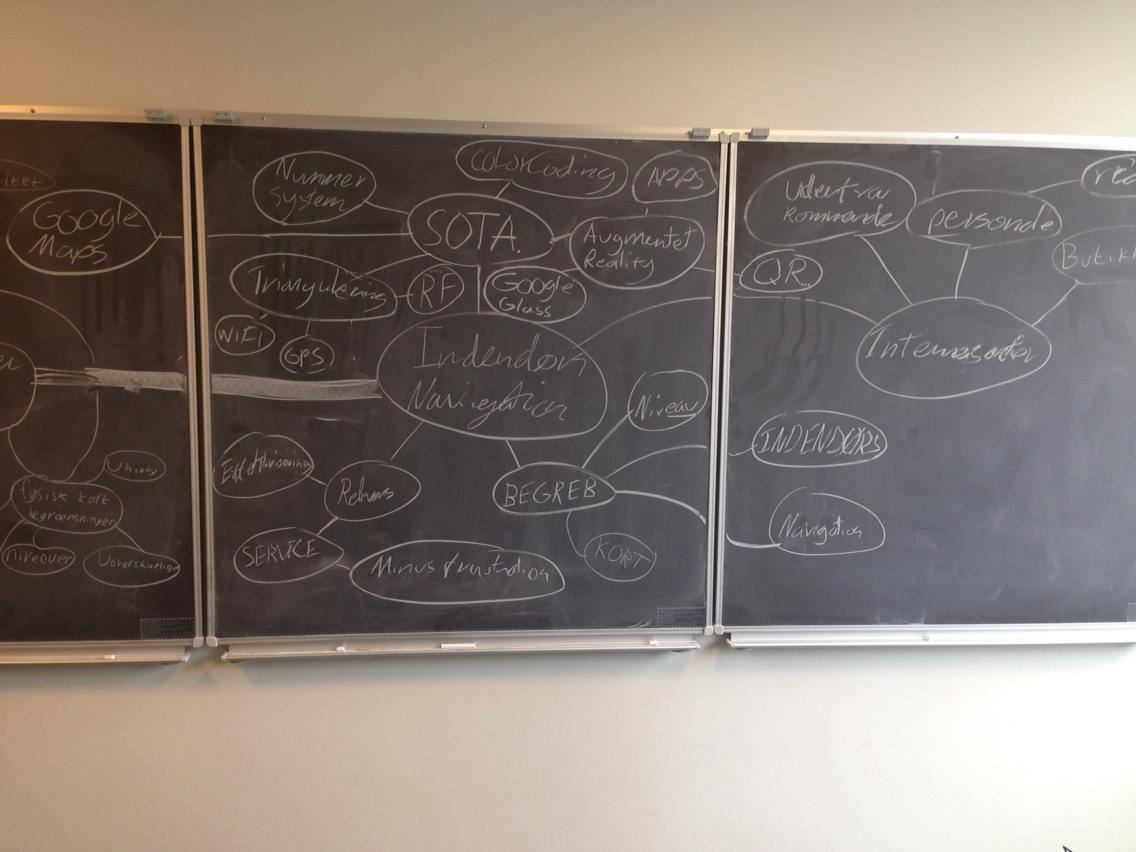
\includegraphics[width=\textwidth]{Images/1.jpg}
                \caption{BAH}
                \label{4}
            \end{minipage}
            \begin{minipage}{0.45\textwidth}
                \centering
                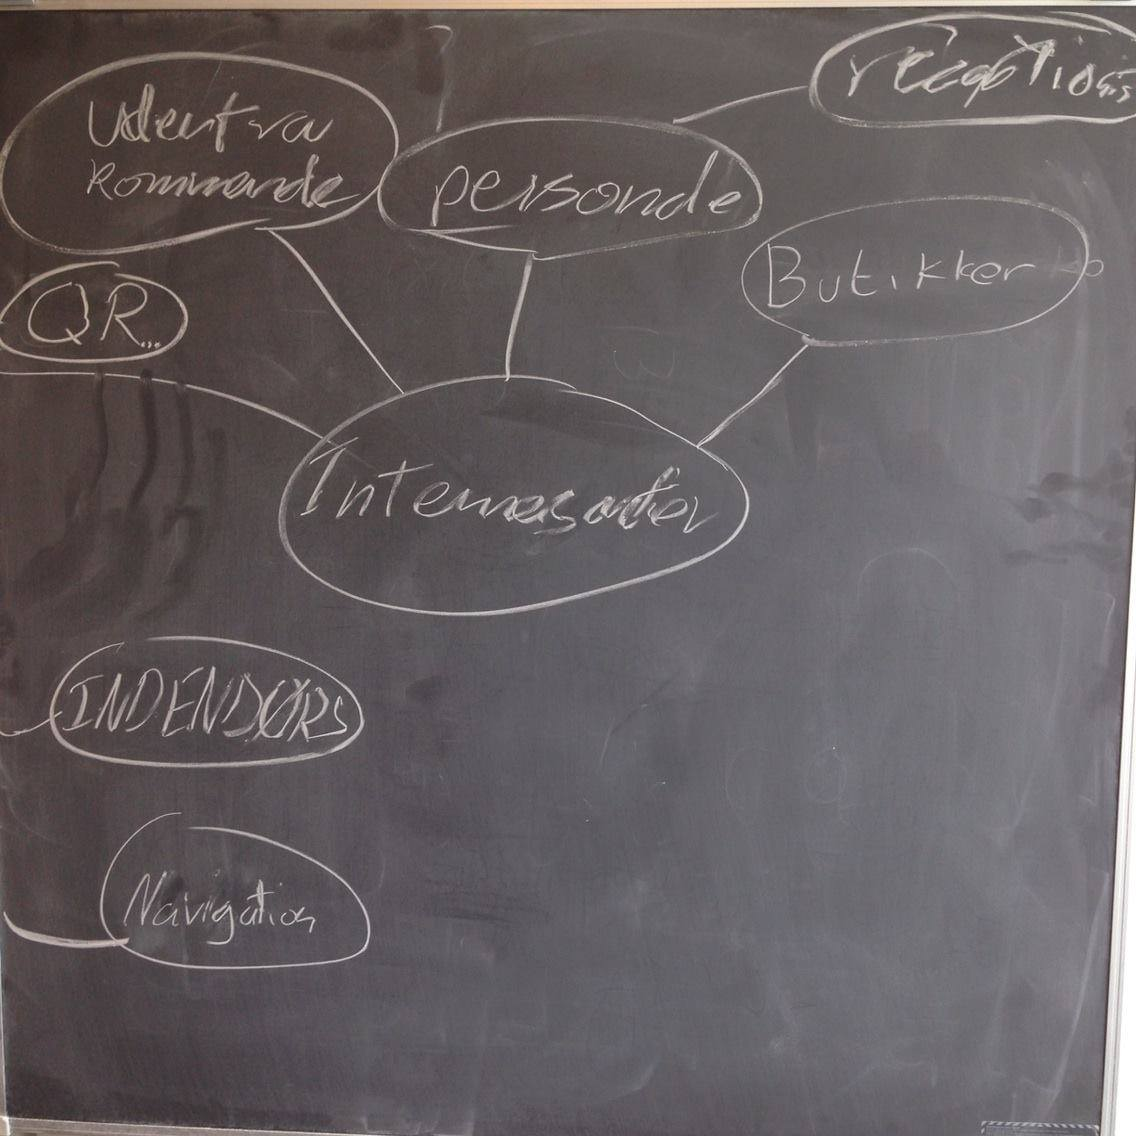
\includegraphics[width=\textwidth]{Images/3.jpg}
                \caption{BAH}
                \label{4}
            \end{minipage}
            \begin{minipage}{0.45\textwidth}
                \centering
                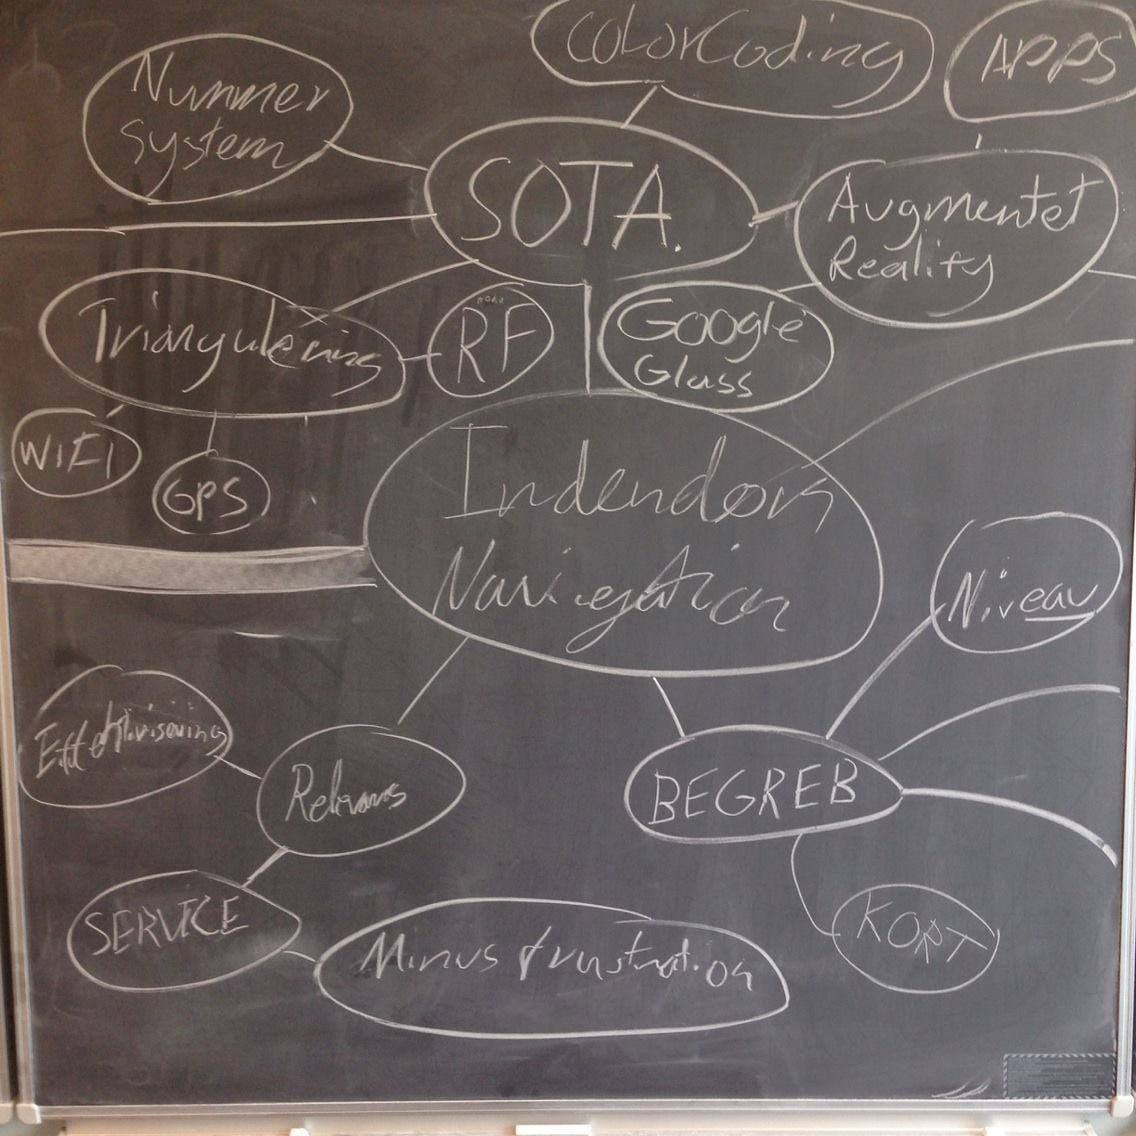
\includegraphics[width=\textwidth]{Images/4.jpg}
                \caption{BAH}
                \label{4}
            \end{minipage}
            \begin{minipage}{0.45\textwidth}
                \centering
                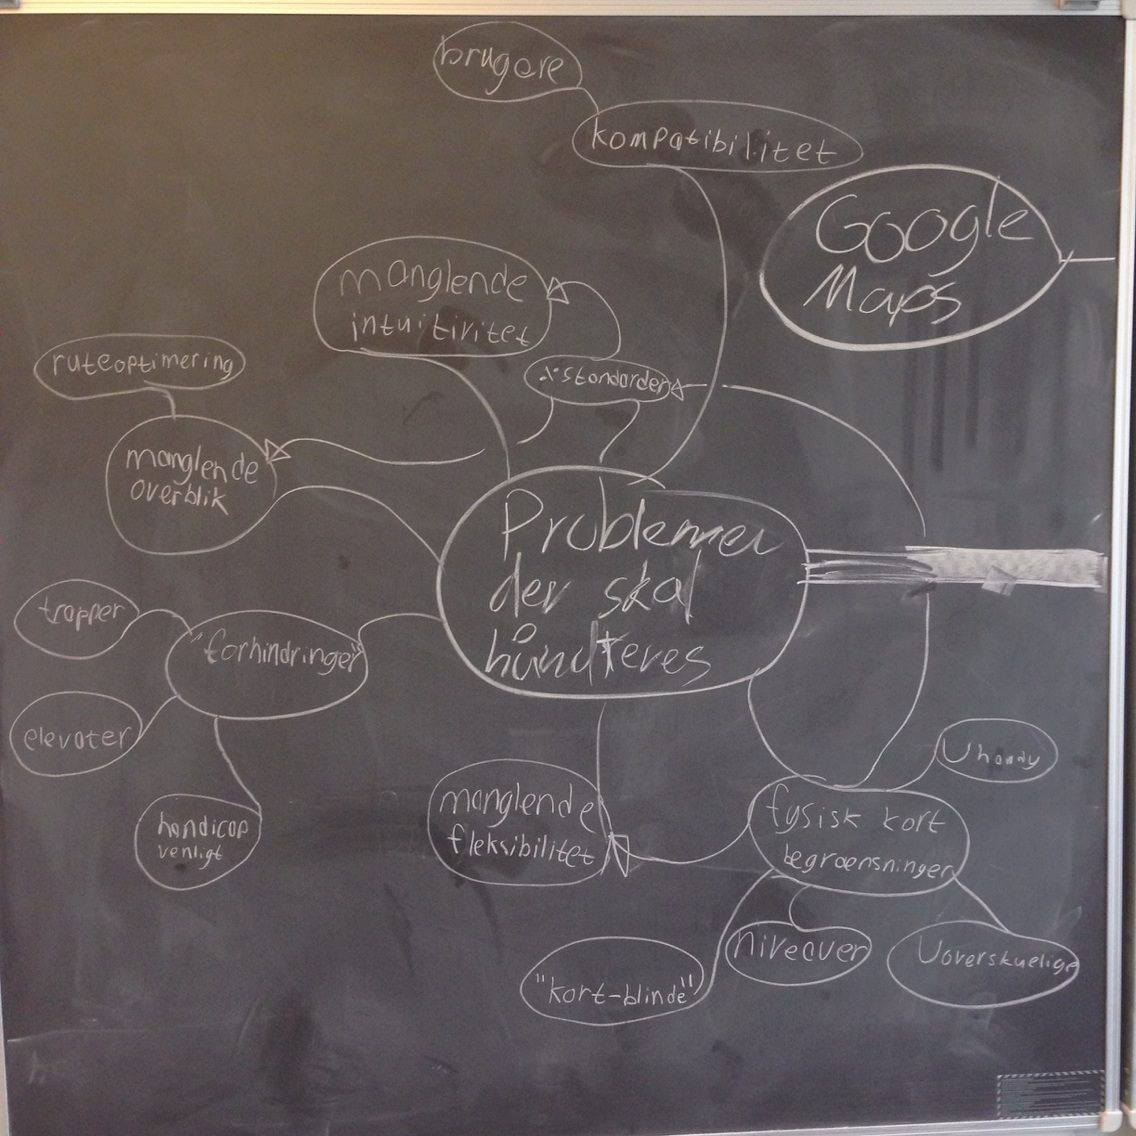
\includegraphics[width=\textwidth]{Images/7.jpg}
                \caption{BAH}
                \label{4}
            \end{minipage}
        \end{figure}

        \subsection{Tegninger}
        Under mange af vores diskussioner, har vi illustreret det for gruppen på tavlen, så alle kunne være  med og her er et af ex. på vores diskussion omkring håndtering af "Floors", der er blevet lavet mange gode ting på tavlen, men ikke alle ting er der blevet taget billeder af.

        \begin{figure}[ht!]
            \centering
            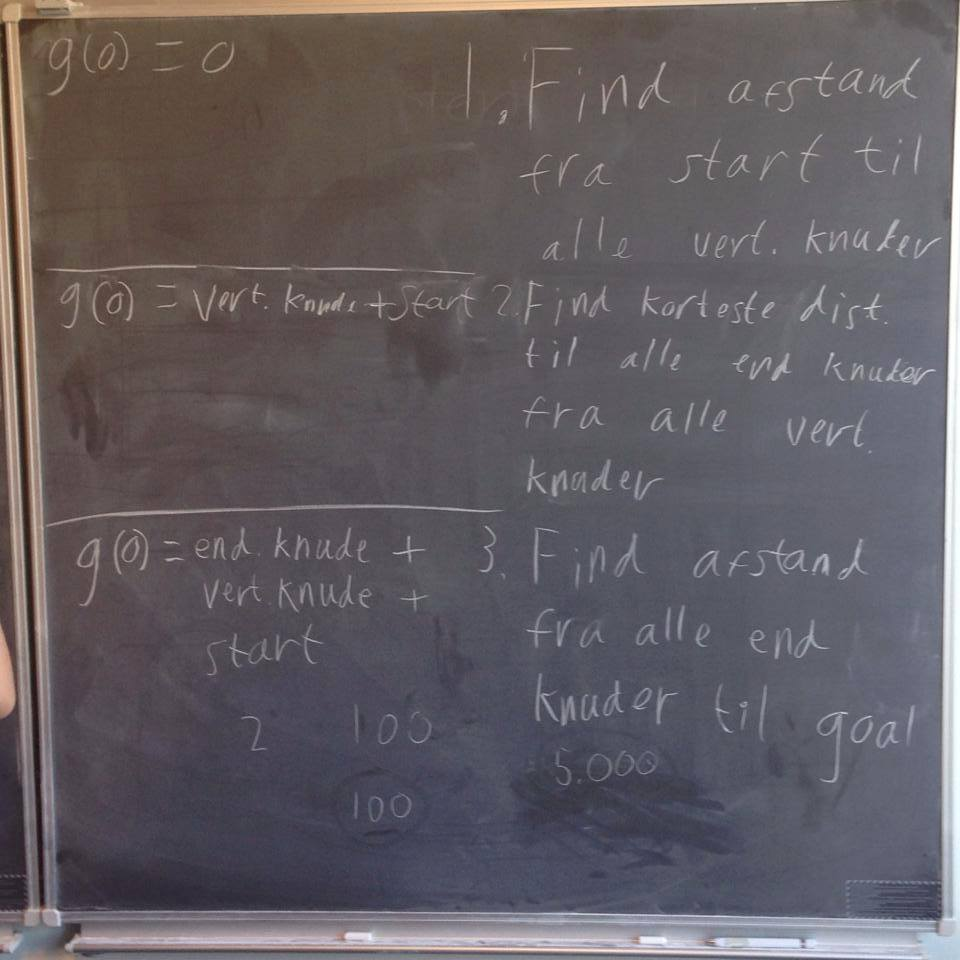
\includegraphics[width=0.5\textwidth]{Images/5.jpg}
            \caption{BAH}
            \label{4}
        \end{figure}

        \begin{figure}[ht!]
            \centering
            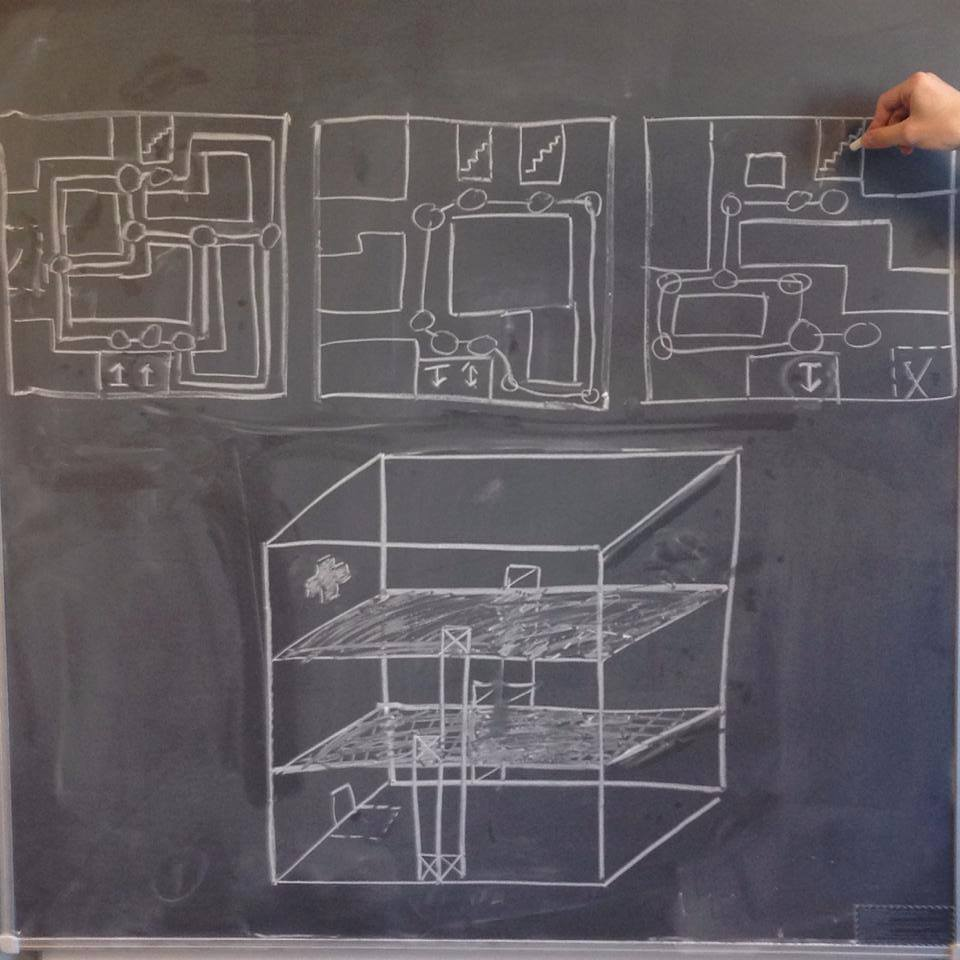
\includegraphics[width=0.5\textwidth]{Images/6.jpg}
            \caption{BAH}
            \label{4}
        \end{figure}


        \subsection{Problemformuleringer}
        For at lave indledningen til den initierende problemstilling var vi nødt til først at have et indgående kendskab til selve problemstillingen. Derfor startede vi med at analysere den formulerede problemstilling. På den måde undersøgte og afdækkede vi problemstillingen og fik det fornødne kendskab der var nødvendigt for at skrive den førnævnte indledning.\\
        Da vi skulle formulere indledningen til den initierende problemstilling, tog vi udgangspunkt i den viden vi havde opnået og brugte denne til at argumentere for vores problemstilling og det var nødvendigt at undersøge denne. Den argumentation vi benyttede bestod bland andet i, at vi drog paralleller til andre lignende problemstillinger, der var blevet løst (udendørs navigation forbedret via GPS navigation), for derefter at argumentere for at den samme problemstilling eksisterede i vores situation (indendørs navigation).

        \subsection{Rapportstrukturering}

        Vi var meget opmærksomme på at rapportstrukturen var skelettet i vores projekt, og det blev derfor prioteret meget højt igennem hele forløbet. Vi kunne med fordel have holdt en smule mere struktur på vores røde tråd, for at have undgået at den blev uddateret.


        \subsection{Andet}
        Under materialle læsning, sendte vi en gruppe ud på Syghus Nord Aalborg, for at tage billeder af hvordan navigeringen foregik, såsom farve kode, kort og skilte.

        Der har ikke været en person, der blev udpeget at været projektleder, istedet har vi været meget demokratiske. Tilsidst i projekt forløbet tog nogle gruppemedlem rollen, som projektleder for en dag, hvis rolle var at skulle styr på hvad der var lavet og hvad der stadig manglede at blivet lavet. Beslutninger har været mere enstemmige, men beslutningerne har også først været taget efter længere diskussioner.

    \section{Syntese - Gode råd til P2}
    Hvis jeres vurdering og analyse skal bidrage til at forbedre jeres evne til at håndtere det 
    problemorienterede og projektorganiserede gruppearbejde, skal I til slut konkretisere jeres 
    erfaringer i nogle ’Gode råd’ til jer selv og jeres medstuderende. En god måde at formulere sådanne 
    gode råd på er som en *start-stop-fortsæt*-liste, dvs. en liste med følgende tre sektioner: 
    Dette vil vi begynde at gøre i P1, som vi ikke gjorde i P0 
    Dette vil vi ikke gøre i P1, som vi gjorde i P0 
    Dette vil vi fortsætte med at gøre (gerne anderledes og bedre) i P1, som vi også gjorde i P0 

\end{document}